
\chapter{Introdução}

As correias são elementos de transmissão amplamente utilizados na indústria para transferir potência entre eixos, encontrando aplicação em equipamentos diversos como motores, compressores, bombas, ventiladores, máquinas agrícolas e sistemas de transporte. Sua versatilidade permite uso desde pequenos eletrodomésticos até grandes instalações industriais.

Entre as principais vantagens das correias destacam-se a operação silenciosa, absorção de vibrações, baixo custo de manutenção e facilidade de instalação. Estas características tornam as transmissões por correias uma solução prática e econômica para diversas aplicações mecânicas.

O presente trabalho aborda os critérios e metodologias para a escolha adequada de correias em projetos de engenharia mecânica, considerando fatores como tipo de aplicação, potência a ser transmitida, condições operacionais e requisitos de disposição.


\begin{figure}[h]
	\centering
	\caption{Aplicação automotiva de correias}
    \label{correia_carro}
	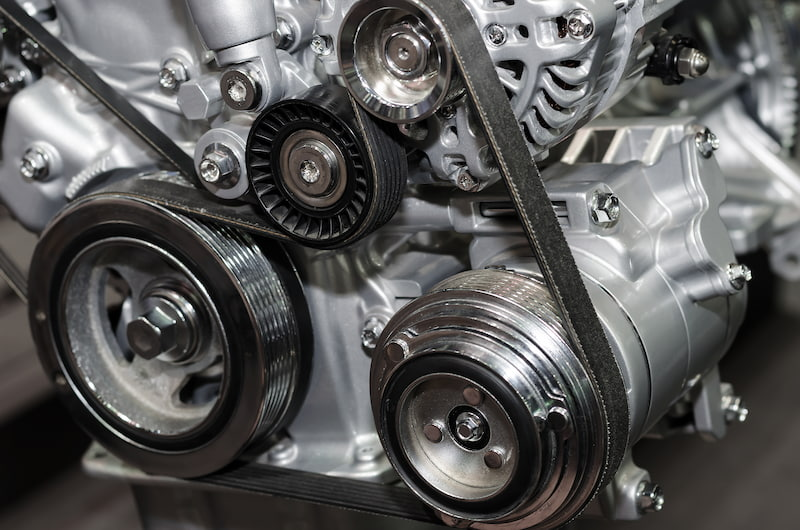
\includegraphics[scale=0.5]{Imagens/correia_carro.jpg}
	\fonte{\cite{correia_carro}}
\end{figure}